\documentclass[a4paper, 11pt]{article}

\usepackage[top=2cm, bottom=2cm, left=2cm, right=2cm]{geometry}
\usepackage[utf8]{inputenc}
\usepackage[T1]{fontenc}
\usepackage{indentfirst}

% Multiple columns
\usepackage{multicol}
\setlength{\columnseprule}{1pt} % separation line between columns

% Colors
\usepackage[usenames,dvipsnames]{xcolor}
\definecolor{dkgreen}{rgb}{0,0.6,0}
\definecolor{steelblue}{rgb}{0.16,0.37,0.58}
\definecolor{gray}{rgb}{0.5,0.5,0.5}
\definecolor{mauve}{rgb}{0.58,0,0.82}
\definecolor{blue}{rgb}{0,0,0.7}
\definecolor{shadecolor}{rgb}{0.96,0.96,0.96}
\definecolor{TFFrameColor}{rgb}{0.96,0.96,0.96}
\definecolor{TFTitleColor}{rgb}{0.00,0.00,0.00}
\definecolor{lightred}{rgb}{1,0.96,0.96}
\definecolor{darkred}{rgb}{0.85,0.33,0.31}
\definecolor{lightblue}{HTML}{EBF5FA}
\definecolor{lightblue2}{HTML}{E3F2FA}
\definecolor{darkblue}{HTML}{D2DCE1}
\definecolor{lightyellow}{HTML}{FFFAE6}
\definecolor{darkyellow}{HTML}{FAE6BE}

\usepackage{hyperref}
\hypersetup{
	colorlinks=true,	% false: boxed links; true: colored links
	linkcolor=black,	% color of internal links
	urlcolor=blue,		% color of external links
	citecolor=blue
}

% Figures & graphics
\usepackage{graphicx}	% import graphics
\usepackage{wrapfig}	% wrap text around figures
\usepackage{subcaption} % subfigures

% Colored frames
\usepackage{mdframed}
\usepackage{framed}

\newenvironment{framehint}{%
	\begin{mdframed}[backgroundcolor=lightblue, linecolor=darkblue]%
}{\end{mdframed}}

\newenvironment{framehint2}{%
	\begin{mdframed}[backgroundcolor=lightblue2, linecolor=darkblue]%
}{\end{mdframed}}

\newenvironment{framewarning}{%
	\begin{mdframed}[backgroundcolor=lightyellow, linecolor=darkyellow]%
}{\end{mdframed}}

\newenvironment{frameurgent}{%
	\begin{mdframed}[backgroundcolor=lightred, linecolor=darkred]%
}{\end{mdframed}}

% Leftbar
\newlength{\leftbarwidth}
\setlength{\leftbarwidth}{1pt}
\newlength{\leftbarsep}
\setlength{\leftbarsep}{10pt}

\newcommand*{\leftbarcolorcmd}{\color{gray}}

\renewenvironment{leftbar}{%
    \def\FrameCommand{{\leftbarcolorcmd{\vrule width \leftbarwidth\relax\hspace {\leftbarsep}}}}%
    \MakeFramed {\advance \hsize -\width \FrameRestore }%
}{%
    \endMakeFramed
}

% Code listings
\usepackage{listings}
\lstset{
	language=java,
	basicstyle=\scriptsize,
	numbers=left,                   % where to put the line-numbers
  	numberstyle=\tiny\color{gray},
	commentstyle=\color{steelblue},
	stringstyle=\color{BrickRed},
	backgroundcolor=\color{shadecolor},
    keywordstyle=\color{OliveGreen},
	frame=single,                   % adds a frame around the code
 	rulecolor=\color{black},
	emph={},
	emphstyle=\color{mauve},
	morekeywords=[2]{obside@obsideb},
	keywordstyle={\color{black}},
	keywordstyle=[2]{\color{dkgreen}},
	showstringspaces=false,
  	tabsize=4,
	moredelim=[is][\small\ttfamily]{/!}{!/},
	breaklines=true
}

% Title page
\title{
	\textbf{Software Architecture}\\
    \Large{Assignment 1 - Design Patterns}
}
\date{\today}

\begin{document}
\maketitle
\newpage

\tableofcontents
\newpage

\section{Exercise 1: Find instances of Design Patterns}

\subsection{Singleton}

\subsection{Abstract Factory}

\subsection{Observer}

\subsection{Adapter}

\subsection{Visitor}

\newpage

\section{Exercise 2: Recognise Design Patterns}

First of all, please find below a simplified class diagram to visualise
more easily how the different classes interact.\\

\begin{figure}[h!]
    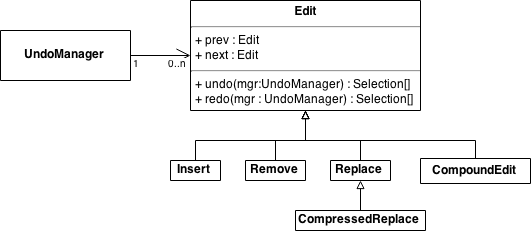
\includegraphics[width=0.8\textwidth]{images/ex2.png}
    \centering
    \caption{Exercise 2 Class Diagram}
\end{figure}

The inner classes \emph{Edit}, \emph{Insert}, \emph{Remove}, \emph{Replace},
\emph{CompressedReplace}, \emph{CompoundEdit} are part of an implementation of
the Command design pattern which is a behavioural pattern. \emph{Edit} is an
abstract class that all commands inherits. Each command must implement an
\emph{undo()} and a \emph{redo()} action. By using this pattern, each operation
applied to a buffer (e.g. inserting text, removing text) is instantiated
as a class implementing the \emph{Edit} interface so that they can be
easily saved in queues in order to \emph{undo()} or \emph{redo()} them.
Without this pattern, undo and redo could be implemented by saving the
content of the buffer after each operation, but that would be more
expensive memory-wise.\\

The \emph{Edit} abstract class and its children are part of a composite
design pattern, which is a structural pattern. In this implementation,
there are no leafs, only composite elements (\emph{Edit} and its
children). This pattern is used here in order to retrieve the previous
and next \emph{Edit}, which is useful for implementing the redo and undo
queues.
\newpage

\section{Exercise 3: Coupling \& Cohesion}

\subsection{Levels of coupling and cohesion}

\textbf{Cohesion} refers to how related attributes and methods are
within a class and if they are responding to the class' intention.
\textbf{High cohesion}, which is preferable, means that a class does one
specific job well. Low cohesion, which should be avoided, means that the
class is not focused on one thing and could be refactored. For example,
an \emph{User} class containing attributes such as the name or the email
address and methods for sending messages to other users has a low
cohesion, since message handling could be refactored and done by other
classes.\\

\textbf{Coupling} refers to the dependencies between classes. Highly
coupled classes cannot be used independently, consequently, changes to
those classes are difficult to make without having to modify all the
dependent classes. It's also hard to reuse and test classes with high
coupling because all the dependencies must be carried with them. So, we
should try to have \textbf{low coupling} between the modules in our
programms.

\subsection{Cohesion in jEdit}

\subsubsection{MiscUtilities}

\emph{MiscUtilities} has a coincidental type of cohesion, which
corresponds to low cohesion. As the class' name implies, it contains
miscellaneous tools: the developers did not know where to put them, so
they put them all in one big class with no relation between the members.
Some possible improvements below.

\begin{itemize}\itemsep1pt
    \item A first simple step to improve the situation would be to group
    together all related methods (e.g. paths, backup) to achieve logical
    cohesion.

    \item One other improvement would be to move methods which are used only
    once where they are called (e.g. \emph{canonPath()} is used only in
    \emph{FileVFS}`s \emph{canonPath()} method).

    \item One could also see paths as potential objects, instead of directly
    manipulating \emph{Strings}. Then, a \emph{Path} class could be
    created, and related methods could be moved into it (and they would
    not be static anymore).

    \item This is more related to code smell than cohesion, but it seems that
    some methods (e.g. \emph{isAbsolutePath()}) are useless since they
    already exist in the JDK (\emph{isAbsolute()}).
\end{itemize}

\subsubsection{GUIUtilities}

\emph{GUIUtilities} has a logical type of cohesion, which is in the
lower part of the cohesion spectrum. This class contains methods related
to GUI handling (e.g. loading an icon, creating a menu item, creating a
toolbar). Here are some improvements which could be made :

\begin{itemize}\itemsep1pt
    \item As stated previously, methods should not be placed here, but with
    their related class based on criteria such as needed parameters, or return
    types. For example, \emph{loadMenuItem()} returns a \emph{JMenuItem} and
    could be placed in this class.

    \item It seems strange to have \emph{SplashScreen} methods globally
    accessible and placed in \emph{GUIUtilities}, since the splash screen
    should be shown only once in the application's lifecycle. Moreover,
    these methods could have been moved into jEdit's \emph{SplashScreen}
    class. The \emph{SplashScreen} should have been instantiated in the
    only part of the application which needs it: \emph{jEdit}'s
    \emph{main()} method. Finally, why is there a jEdit
    \emph{SplashScreen} class when there is already a way of doing it in
    Swing? It can even be handled by using the \emph{SplashScreen-Image}
    option in the JAR's manifest file. \cite{cite:swingSplash}
\end{itemize}

\begin{framehint2}
    \textbf{N.B.} On a side note, since we are talking about UI, tools like
    SWIXML or JavaFX could be used to generate the UI by parsing XML files.
    The main advantage would be to separate the UI from the program's logic.
\end{framehint2}

\subsubsection{VFSFile}

All attributes from \emph{VFSFile} are primitive data types or part of
the JDK (\emph{String}) and are related to a file properties (e.g. name, path,
length). this class' methods also seem to be all related to handling files.
So, this class is an example of functional cohesion (high cohesion).

\begin{framewarning}
    While the cohesion seem to be high does not mean than no improvements can
    be made.
    For example, the file's colour is handled by a \emph{getColour()} method which
    retrieve a colour based on the VFS. Colour is more related to the UI than
    file handling, and could be computed elsewhere.
    By computing the colour in \emph{VFSFile}, it ties this class to one
    possible representation of the UI. On the other hand, this is not harmful in
    this case, since the class could be reused elsewhere and the code related to
    colour deleted without too much effort, if not used. Furthermore, the
    current solution is simple to use, and separating colour from
    \emph{VFSFile} could cause unnecessary efforts for no real benefit.
\end{framewarning}

\subsection{Coupling in jEdit}

The \emph{jEdit} and \emph{GUIUtilities} classes seem to be highly
coupled, since they cannot be used independently :

\begin{itemize}\itemsep1pt
    \item \emph{jEdit} relies on static methods from \emph{GUIUtilities} (e.g.
    \emph{showSplashScreen()}, \emph{advanceSplashProgress()})

    \item \emph{GUIUtilities} relies on static methods from \emph{jEdit} (e.g.
    \emph{getProperty()}, \emph{setProperty()})
\end{itemize}

These two classes share global data through static methods, it implies
that this is a case of common coupling. Using static methods can lead to
problematic situations. First of all, dependencies between classes when
using static methods are hidden, since they do not appear as a class' attribute
and are not part of a method's parameters (they are not visible in the
class' interface). Static methods can also be accessed from anywhere, it
is probably safe if they are only used to access data and not modify it,
but that does not seem to be the case here (e.g.
\emph{jEdit.setProperty()}). Being able to modify data from anywhere in
the application makes testing difficult: if a class need to access a
specific static data, and this data can be anything at any point in the
application, then it is impossible to test efficiently this class
because the state of the application is undefined. \cite{cite:jenkovDependencies}\\

Below are some ideas to reduce coupling between these 2 classes :

\begin{itemize}\itemsep1pt
    \item get rid of \emph{GUIUtilities}, and use some other way of handling UI
    (previously talked about UI generated from XML files);

    \item a more simple improvement would be to move the splashscreen
    instantiation to \emph{jEdit}'s main method, since it is the only place in
    the application that a splashscreen should be called.
    All the methods related to the splashscreen in \emph{GUIUtilities} should be
    moved to the intended class (\emph{SplashScreen});

    \item properties being globally accessible could be useful, but there should
    be restrictions on who can modify them
\end{itemize}

\newpage


\begin{thebibliography}{10}
% TODO \bibitem{cite:REF} \emph{TITLE}, FROM, AUTHOR, \href{URL}{URL}

\bibitem{cite:headfirst} \emph{Head First Design Patterns}, Eric Freeman, Elisabeth Robson, Bert Bates, Kathy Sierra, O'Reilly, October 2004

\bibitem{cite:plSingletonGlobal} \emph{Singleton Design Pattern vs. Global Variable}, Programming in the Large, Eddie Burris, \href{http://programminglarge.com/singleton-design-pattern-vs-global-variable/}{http://programminglarge.com/singleton-design-pattern-vs-global-variable/}

\bibitem{cite:soSingleton} \emph{What is so bad about singletons?}, Stack Overflow, \href{https://stackoverflow.com/questions/137975/what-is-so-bad-about-singletons}{https://stackoverflow.com/questions/137975/ what-is-so-bad-about-singletons}

\bibitem{cite:seGlobal} \emph{Why is Global State so Evil?}, Programmers Stack Exchange, \href{https://programmers.stackexchange.com/questions/148108/why-is-global-state-so-evil}{https://programmers.stackexchange .com/questions/148108/why-is-global-state-so-evil}

\bibitem{cite:soAdapterDiff} \emph{How do the Proxy, Decorator, Adapter, and Bridge Patterns differ?}, Stack Overflow, \href{https://stackoverflow.com/questions/350404/how-do-the-proxy-decorator-adapter-and-bridge-patterns-differ}{https://stackoverflow.com/questions/350404/how-do-the-proxy-decorator-adapter-and-bridge-patterns-differ}

\bibitem{cite:javaDocWindowAdapter} \emph{Class WindowAdapter}, Java SE 8 documentation, \href{http://docs.oracle.com/javase/8/docs/api/java/awt/event/WindowAdapter.html}{http://docs.oracle.com/javase/8/docs/api /java/awt/event/WindowAdapter.html}

\bibitem{cite:swingSplash} \emph{How to Create a Splash Screen}, Oracle Java Tutorials, \href{http://docs.oracle.com/javase/tutorial/uiswing/misc/splashscreen.html}{http://docs.oracle.com/javase/tutorial /uiswing/misc/splashscreen.html}

\bibitem{cite:jenkovDependencies} \emph{Understanding Dependencies}, Jakob Jenkov, \href{http://tutorials.jenkov.com/ood/understanding-dependencies.html}{http://tutorials.jenkov.com/ood/understanding-dependencies.html}
\end{thebibliography}

\end{document}
